\section{Geometry of a Node Element}\label{sec:element-geometry}

\begin{figure}
    \centering
    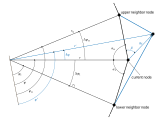
\includegraphics{img/model_development/element_geometry}
    \caption{Geometry Overview of a Node Element}
    \label{fig:model_development/element_geometry}
\end{figure}

Each node of the surface line forms an element with its neighbors, not to be confused with finite element approaches.
Its geometry and important quantities are displayed in \autoref{fig:model_development/element_geometry}.
Their relations used in following calculations will be derived in this section.

To avoid writing numeric indices everywhere, the quantities belonging to the currently regarded node will be written without any index.
The indices $\ldots_{\Upper}$ and $\ldots_{\Lower}$ are used to denote the upper and lower neighbor of this node.

The surface distance between the adjacent nodes is calculated using the cosine law as in \autoref{eq:surface-distance}, with the angle distances $\Diff\Angle_{\Upper} = \Angle_{\Upper} - \Angle$ and $\Diff\Angle_{\Lower} = \Angle - \Angle_{\Lower}$.
The distances are always positive.

\begin{subequations}
    \begin{align}
        \SurfaceDistance_{\Upper} &= \sqrt{\Radius_{\Upper}^2 + \Radius^2 - 2\Radius_{\Upper}\Radius \cos \Diff\Angle_{\Upper}} \\
        \SurfaceDistance_{\Lower} &= \sqrt{\Radius_{\Lower}^2 + \Radius^2 - 2\Radius_{\Lower}\Radius \cos \Diff\Angle_{\Lower}}
    \end{align}
    \label{eq:surface-distance}
\end{subequations}

The angles between the surface lines and the radius vector (surface-radius-angles) are calculated given the node coordinates using the cosine law \autoref{eq:surface-radius-angles}.
Cosine law has been chosen over sine law due to its support for angles from 0 to $\PI$ rather than $-\frac\PI2$ to $\frac\PI2$.
However, when undercuts occur in the particle surface $\Diff\Angle_{\Upper}$ or $\Diff\Angle_{\Lower}$ may be negative, then the sign of the surface radius angle must equal that of the angle distances.
This negative angle is required for the volume partial differential to change its sign accordingly as derived in \autoref{sec:surface-evolution}.

\begin{subequations}
    \begin{align}
        \SurfaceRadiusAngle_{\Upper} &= \sign(\Diff\Angle_{\Upper}) \cdot \arccos \left[ \frac{\Radius_{\Upper}^2 - \Radius^2 - \SurfaceDistance_{\Upper} ^ 2}{-2 \Radius \SurfaceDistance_{\Upper}} \right] \\
        \SurfaceRadiusAngle_{\Lower} &= \sign(\Diff\Angle_{\Lower}) \cdot \arccos \left[ \frac{\Radius_{\Lower}^2 - \Radius^2 - \SurfaceDistance_{\Lower} ^ 2}{-2 \Radius \SurfaceDistance_{\Lower}} \right]
    \end{align}
    \label{eq:surface-radius-angles}
\end{subequations}

During simulation of sintering, the particle surface evolves by shifting the nodes to a new location in each time step.
The new coordinates after shifting along a vector $\Step\Shift$ which is directed under an angle of $\SurfaceVectorAngle$ with the upper surface line are calculated using cosine and sine law as in \autoref{eq:new-node-coordinates}.
The latter allows here negative changes in the angle coordinate $\Step\Angle$, which are to be expected much smaller than $\frac\PI2$.
The shift vector is for now arbitrary, but will be concretized in \autoref{sec:surface-evolution}.

\begin{subequations}
    \begin{align}
        \Radius' &= \Radius^2 + {\Step\Shift}^2 - 2 \Radius\Step\Shift \cos \left( \SurfaceRadiusAngle_{\Upper} + \SurfaceVectorAngle_{\Upper} \right) \\
        \Angle' &= \Angle + \Step\Angle = \Angle + \arcsin \left[ \frac{\sin \left( \SurfaceRadiusAngle_{\Upper} + \SurfaceVectorAngle_{\Upper} \right) }{\Radius'} \Step\Shift \right]
    \end{align}
    \label{eq:new-node-coordinates}
\end{subequations}

For the sake of sintering behavior analysis and evaluation of numerical error the volume of a particle has to be determined (actually area due to 2D).
This is done by summing over all element triangles as in \autoref{eq:particle-volume}, where $\Nodes$ is the set of all nodes the particle consists of.
Note, that if undercuts occur this equation is still correct since the respective elements will be counted negative as then $\sin \Diff\Angle_{\Upper} < 0$.

\begin{equation}
    \Volume_{\Particle} = \frac12 \sum^{\Nodes} \Radius\Radius_{\Upper} \sin \Diff\Angle_{\Upper}
    \label{eq:particle-volume}
\end{equation}
